\documentclass[a4paper, 11pt,reqno]{article}
\input{/Users/olivierglorieux/Desktop/BCPST/2020:2021/preambule.tex}
\usepackage{enumitem}
\geometry{hmargin=2.5cm, vmargin=2.5cm}
\lstset{basicstyle=\ttfamily, keywordstyle=\rmfamily\bfseries}
\newif\ifshow
\showtrue

\input{/Users/olivierglorieux/Desktop/BCPST/2021:2022/ifshow.tex}

\author{Olivier Glorieux}


\begin{document}

\title{ Correction DS8}



\begin{exercice}
Les questions de cet exercice sont indépendantes. 
\begin{enumerate}
\item Justifier que $E=\{(x,y,z) \in \R^3\, |\, xyz=0\}$ n'est pas un sous-espace vectoriel de $\R^3$.
\item Soit $F=\{ (x,y,z,t)\in \R^4 \, |\, x+y+z+t=0, 2x+y+z-t=0\}$
Montrer que $F$ est sous-espace vectoriel de $\R^4$ et en donner une base. 

\item Montrer que $((1,2,3),(1,0,1), (2,2,1))$ est une base de $\R^3$.

\item Donner les DL à l'ordre 2 en  0 de $\exp(x),\ln(\cos(x)),\sqrt{1+2x}$ et $\sin(x^2)$ puis  en déduire la limite suivante 
$$\lim_{x\tv 0} \frac{e^x+\ln(\cos(x))-\sqrt{1+2x}}{\sin(x^2)}$$

\end{enumerate}

\end{exercice}

\begin{correction}
\begin{enumerate}
\item $(1,1,0)$ et $(0,0,1)$ appartiennent à $E$ mais $(1,1,0)+(0,0,1) = (1,1,1)$ n'appartient pas à $E$ donc $E$ n'est pas stable par combinaisons linéaires en particulier \conclusion{ $E$ n'est pas un sev de $\R^3$. }
\item Montrons que $F$ est un sev. (Comme dit en TD la deuxième partie suffit, en montrant que c'est le sev engendré par une certaine famille de vecteurs, mais bon, il faut savoir faire aussi ca) 
Tout d'abord, $(0,0,0,0)\in F$ car $0+0+0+0=0$...

Soit $u_1, u_2 \in F$ et $\lambda \in R$. On  pose $u_1 =(x_1,y_1,z_1,t_1) $et $u_2 =(x_2,y_2,z_2,t_2) $ on a alors : 
\begin{align*}
u_1 +\lambda u_2 &=(x_1,y_1,z_1,t_1) +\lambda (x_2,y_2,z_2,t_2) \\
								&= (x_1+\lambda x_2,y_1+\lambda y_2,z_1+\lambda z_2,t_1+\lambda t_2) 
\end{align*}

Et 
\begin{align*}
x_1+\lambda x_2 + y_1+\lambda y_2 +z_1+\lambda z_2 + t_1+\lambda t_2 &= (x_1 +y_1+z_1+t_1) +\lambda  (x_2 +y_2+z_2+t_2)\\
&=0 +\lambda 0 \text{\quad Car $u_1\in F$ et $u_2 \in F$}\\
&=0
\end{align*}
\begin{align*}
2(x_1+\lambda x_2) + y_1+\lambda y_2 +z_1+\lambda z_2 -( t_1+\lambda t_2) &= (2x_1 +y_1+z_1-t_1) +\lambda  (2x_2 +y_2+z_2-t_2)\\
&=0 +\lambda 0 \text{\quad Car $u_1\in F$ et $u_2 \in F$}\\
&=0
\end{align*}

Finalement, $F$ est stable par combinaisons linéaires. 
\conclusion{ $F$ est un sous-espace vectoriel de $\R^4$}

Par ailleurs $(x,y,z,t)\in F \equivaut 
\left\{ \begin{array}{rr}
x+y+z+t&=0\\
2x+y+z-t&=0\\
\end{array}\right.\equivaut 
\left\{ \begin{array}{rr}
x+y+z+t&=0\\
-y-z-3t&=0\\
\end{array}\right.
$ 
On obtient alors 
$$\left\{ \begin{array}{rr}
x+y&=-z-t\\
y&=-z-3t\\
\end{array}\right. \equivaut \left\{ \begin{array}{rr}
x&=2t\\
y&=-z-3t\\
\end{array}\right. 
$$
Donc 
\begin{align*}
F&=\{ (2t,-z-3t,z,t)\, |\, (z,t)\in \R^2\}\\
&=\{ t(2,-3,0,1) +z(0,-1,1,0)\, |\, (z,t)\in \R^2\}\\
&= \Vect((2,-3,0,1),(0,-1,1,0))
\end{align*}
$((2,-3,0,1),(0,-1,1,0))$ est donc une famille génératrice de $F$. Comme les deux vecteurs ne sont pas proportionnels c'est une famille libre. 

Ainsi 
\conclusion{ $((2,-3,0,1),(0,-1,1,0))$ est une base de $F$}

\item Montrons que la famille $((1,2,3),(1,0,1), (2,2,1))$ est une famille libre. 

Soit $(\lambda_1,\lambda_2 \lambda_3)\in \R^3$ trois réels tels que

$$\lambda_1(1,2,3)+ \lambda_2(1,0,1)+ \lambda_3(2,2,1) =(0,0,0)$$
On a alors 

$$ \left\{ \begin{array}{crc}
\lambda_1 + &\lambda_2+ 2\lambda_3 &=0\\
2\lambda_1 + & + 2\lambda_3 &=0\\
3\lambda_1 + &\lambda_2 + 1\lambda_3 &=0\\
\end{array}\right. \equivaut 
\left\{ \begin{array}{crc}
\lambda_1 + &\lambda_2+ 2\lambda_3 &=0\\
 &-2\lambda_2  -2\lambda_3 &=0\\
&-2\lambda_2 -5\lambda_3 &=0\\
\end{array}\right. 
\equivaut 
\left\{ \begin{array}{crc}
\lambda_1 + &\lambda_2+ 2\lambda_3 &=0\\
 &-2\lambda_2  -2\lambda_3 &=0\\
& -3\lambda_3 &=0\\
\end{array}\right. 
$$
Ainsi le système est de rang 3 avec 3 inconnues. Il est donc de Cramer et admet une unique solution, à savoir $(0,0,0)$ car le système est homogéne. 
Ainsi 
\conclusion{ La famille $((1,2,3),(1,0,1), (2,2,1))$  est libre}
Or 
$\Card(((1,2,3),(1,0,1), (2,2,1)) = 3 =\dim(\R^3)$
\conclusion{ La famille $((1,2,3),(1,0,1), (2,2,1))$  est une base de $\R^3$}


\item $$\exp(x) = 1+x+\frac{x^2}{2} +o(x^2)$$
$\cos(x) = 1-\frac{x^2}{2} +o(x^2)$ et $\ln(1+u) = u -\frac{u^2}{2} +o(u)$
donc $$\ln(\cos(x)) = \ln(1+\cos(x)-1)= -\frac{x^2}{2} +o(x^2)$$

$$\sqrt{1+2x} = 1+x -\frac{1}{2}x^2+o(x^2)$$


$$\sin(x^2)= x^2 +o(x^2)$$

In fine $$e^x+\ln(\cos(x))-\sqrt{1+2x} =  1+x+\frac{x^2}{2}    -\frac{x^2}{2} -(1+x -\frac{1}{2}x^2)+o(x^2) = \frac{x^2}{2} +o(x^2)$$

Donc $ \frac{e^x+\ln(\cos(x))-\sqrt{1+2x}}{\sin(x^2)} \sim_0 \frac{ \frac{x^2}{2} }{x^2 }\sim_0 \frac{1}{2}$
D'où 
\conclusion{ $ \ddp \lim_{x\tv 0} \frac{e^x+\ln(\cos(x))-\sqrt{1+2x}}{\sin(x^2)} =\frac{1}{2}$}

\end{enumerate}
\end{correction}


\begin{exercice}[Agro 2016]
On considère la suite $\left(S_n\right)_{n \in \mathbb{N}^*}$ définie par
$$
\forall n \in \mathbb{N}^*, \quad S_n=\sum_{k=1}^n \frac{\ln k}{k} .
$$
\begin{enumerate}

\item Ecrire une fonction Python \texttt{suiteS} qui prend en argument un entier \texttt{n} et retourne la valeur de $S_n$.
\item Étude de la nature de la suite $\left(S_n\right)_{n \in \mathbb{N}^*}$.
\begin{enumerate}
\item Dresser le tableau de variations de la fonction $f: x \mapsto \frac{\ln (x)}{x}$.
\item Ecrire un script Python  qui permet de tracer et d'afficher le graphe de $f$ entre 1 et 10 pour l'axe des abscisses et -10 et 10 pour l'axe des ordonnées. Sur l'axe des abscisses on prendra 100 points par intervalle de taille 1. 
\item En déduire que, pour tout entier $k$ supérieur ou égal à 4 , on a :
$$
\int_k^{k+1} \frac{\ln (x)}{x} \mathrm{~d} x \leq \frac{\ln (k)}{k} \leq \int_{k-1}^k \frac{\ln (x)}{x} \mathrm{~d} x
$$
\item En déduire l'existence de trois constantes réelles positives $A, B$ et $C$ telles que, pour tout entier naturel $n$ supérieur ou égal à 4 , on ait :
$$
\frac{\ln ^2(n+1)}{2}-A \leq S_n-B \leq \frac{\ln ^2(n)}{2}-C .
$$
\item En déduire la limite de la suite $\left(S_n\right)_{n \in \mathbb{N}^*}$.
\end{enumerate}
\item  Recherche d'un équivalent de $S_n$.
\begin{enumerate}
\item Montrer que $\ln ^2(n+1) \underset{n \rightarrow+\infty}{\sim} \ln ^2(n)$.
\item En déduire que $S_n \underset{n \rightarrow+\infty}{\sim} \frac{\ln ^2(n)}{2}$.

\end{enumerate} 
\item Étude asymptotique de la suite $u$ définie par :
$$
\forall n \in \mathbb{N}^*, \quad u_n=S_n-\frac{\ln ^2(n)}{2}
$$

Soit $g(n) =\frac{\ln^2(n)}{2}$. On note  $\tau_{n,n+1}(g) = \frac{g(n+1)-g(n)}{n+1- n }$. On admet le résultat\footnote{Appelé inégalité des accroissements finis} suivant : $\forall n\in \N^* $ 
$$\inf_{x\in [n,n+1] } g'(x)\leq \tau_{n,n+1}(g) \leq \sup_{x\in [n,n+1] } g'(x)$$

\begin{enumerate}
\item Montrer à l'aide du résultat admis que, pour tout entier $n$ supérieur ou égal à $3, u_{n+1}-u_n \leq 0$.
\item En déduire que la suite $u$ converge. On note $\ell$ sa limite.
\item Conclure que $S_n \underset{+\infty}{=}  \frac{\ln^2(n)}{2} +\ell +o(1)$
\end{enumerate}
%\item 
%On considère la suite $\left(A_n\right)_{n \in \mathbb{N}^*}$ définie par : $\forall n \in \mathbb{N}^*, A_n\ddp =\sum_{k=1}^n(-1)^{k-1} \frac{\ln (k)}{k}$. 
%\begin{enumerate}
%\item  Prouver que pour tout entier naturel non nul $n$, on a
%$$
%A_{2 n}=S_{2 n}-S_n-\ln (2) \sum_{k=1}^n \frac{1}{k} .
%$$
%
%
%On admet qu'il existe un réel $\gamma$ tel que $\ddp \sum_{k=1}^n \frac{1}{k}\underset{+\infty}{=} \ln (n)+\gamma+o(1)$.
%\item En déduire que la suite $\left(A_{2 n}\right)_{n \in \mathbb{N}^*}$ converge et déterminer sa limite en fonction de $\gamma$.
%\item En déduire que la suite $\left(A_{2 n+1}\right)_{n \in \mathbb{N}^*}$ converge et déterminer sa limite en fonction de $\gamma$.
%\item Que peut-on en déduire au sujet de la suite $\left(A_n\right)_{n \in \mathbb{N}^*}$ ?
%\end{enumerate}
\end{enumerate}

\end{exercice}

\begin{correction}
\begin{enumerate}
\item 
\begin{lstlisting}
import math as m
def suiteS(n):
  S=0
  for k in range(1,n+1):
    S+=S+m.log(k)/k
  return(S)
\end{lstlisting}

\item 
\begin{enumerate}
\item $f$ est définie est dérivable sur $D_f=\R_+^*$ et pour tout $x\in D_f$
$$f'(x)= \frac{\frac{1}{x} x -\ln(x)}{x^2} = \frac{1-\ln(x)}{x^2}$$
Ainsi $$f'(x) \geq 0 \equivaut 1-\ln(x)\geq 0 \equivaut \ln(x)\leq 1 \equivaut x\leq e$$
\begin{center}
\begin{tikzpicture}
   \tkzTabInit{$x$ / 1 , $f'(x)$ / 1, $f(x)$ / 1.5}{$0$, $e$, $+\infty$}
   \tkzTabLine{, +, z, -, }
   \tkzTabVar{-/ $-\infty$ , +/ $\frac{1}{e}$, -/ 0}
\end{tikzpicture}
\end{center}
\item
Le script  pourrait etre le suivant 
 \begin{lstlisting}
import matplotlib.pyplot as plt
import math as m
def f(x):
  return(m.log(x)/x))
X=[1+0.01*k  for k in range(900)]
Y=[f(x) for x in X]
plt.plot(X,Y)
plt.ylim(-10,10)
plt.show()
\end{lstlisting}
\item Pour tout entier $k\geq e $ (donc $k\geq 3$) et pour tout $x\in [k,k+1]$ on a par décroissance de $f$ : 
$$f(x) \geq f(k)$$
D'où en intégrant entre $k $ et $k+1$, par positivité de l'intégrale :
$$\ddp \int_{k}^{k+1} f(x) dx\leq \int_{k}^{k+1} f(k) dx$$
et $\ddp \int_{k}^{k+1} f(k) dx= f(k)$ Donc 
$$\int_{k}^{k+1} f(x) dx\leq f(k) $$

De même  tout entier $k$ tel que $k-1\geq e $ (donc $k\geq 4$) et pour tout $x\in [k-1,k ]$ on a par décroissance de $f$ : 
$$f(x) \leq f(k)$$
D'où en intégrant entre $k-1 $ et $k$, par positivité de l'intégrale :
$$\ddp \int_{k-1}^{k} f(x) dx\leq \int_{k-1}^{k} f(k) dx$$
or $\ddp \int_{k-1}^{k}+ f(k) dx= f(k)$ Donc 
$$\int_{k}^{k+1} f(x) dx\leq f(k) $$

D'où pour tout $x\geq 4$:
\conclusion{ $
\ddp \int_k^{k+1} \frac{\ln (x)}{x} \mathrm{~d} x \leq \frac{\ln (k)}{k} \leq \int_{k-1}^k \frac{\ln (x)}{x} \mathrm{~d} x
$}

\item 
On va sommer les inégalités précédentes pour $k$ entre $4$ et $n$. 
Remarquons qu'en utilisant la relation de Chasles on obtient 
$$\sum_{k=4}^n \int_k^{k+1} \frac{\ln(x)}{x}dx = \int_4^{n+1} \frac{\ln(x)}{x} dx \quadet \sum_{k=4}^n \int_{k-1}^{k} \frac{\ln(x)}{x}dx = \int_3^{n} \frac{\ln(x)}{x} dx$$ 

On obtient donc 

$$\int_4^{n+1} \frac{\ln(x)}{x} dx \leq \sum_{k=4}^n \frac{\ln(k)}{k}\leq 
\int_3^{n} \frac{\ln(x)}{x} dx $$
Or, on  a 
\begin{align*}
 \int_4^{n+1} \frac{\ln (x)}{x}  &= [\frac{1}{2}\ln^2(x)]_4^{n+1}\\
 												&= \frac{1}{2}\ln^2(n+1)- \frac{1}{2}\ln^2(4)\\
 												&= \frac{1}{2}\ln^2(n+1)-2\ln^2(2)
\end{align*}
et 
$$\sum_{k=4}^n \frac{\ln(k)}{k} = S_n - \frac{\ln(3)}{3}-\frac{\ln(2)}{2}$$
et enfin
\begin{align*}
 \int_3^{n} \frac{\ln (x)}{x}  &= [\frac{1}{2}\ln^2(x)]_3^{n}\\
 												&= \frac{1}{2}\ln^2(n)- \frac{1}{2}\ln^2(3)
\end{align*}

On peut donc prendre $A= 2\ln^2(2)$, $B= \frac{\ln(3)}{3}+\frac{\ln(2)}{2}$ et  $C= \frac{1}{2}\ln^2(3)$ et on obtient 
\conclusion{ $\ddp \frac{\ln ^2(n+1)}{2}-A \leq S_n-B \leq \frac{\ln ^2(n)}{2}-C .$}
\item $n \tv \frac{\ln^2(n+1)}{2}$ tend vers $+\infty $ en $+\infty$. Ainsi 
par comparaison 
\conclusion{ $\suiteun{S}$ tend vers $+\infty$}


\end{enumerate}
\item \begin{enumerate}
\item On a par définition de $\suiteun{S}$ et $\suiteun{S}$ :
\begin{align*}
u_{n+1} -u_n&= S_{n+1} -\frac{\ln(n+1)^2}{2}- S_n +\frac{\ln^2(n)}{2}\\
					&= \frac{\ln(n+1)}{n+1}- \frac{\ln^2(n+1)-\ln^2(n)}{2}\\
\end{align*}

Utilisons maintenant le résultat admis : 
On a après simplification $$\tau_{n,n+1}(g) =  \frac{\ln^2(n+1) -\ln^2(n)}{2}$$
Et on a $g'(x)=\frac{\ln(x)}{x}$. On a vu que $g'=f$ était décroissante sur $[ 3,+\infty[$
donc pour tout $n\geq 3$ et pour tout $x\in [n,n+1]$ 
$$g'(x) \geq g'(n+1) =  \frac{\ln(n+1)}{n+1}$$
Ainsi l'inégalité des accroissements finis donne pour $n\geq3$

$$ \frac{\ln^2(n+1) -\ln^2(n)}{2} \geq  \frac{\ln(n+1)}{n+1}$$
Autrement dit 
\conclusion{ $\forall n \geq 3, u_{n+1} -u_n\leq 0$}
\item La suite $\suiteun{u} $ est décroissante d'après la question précédente. Montrons qu'elle est minorée. 
D'après la question 1c) on a pour tout $n\geq 3$
\begin{align*}
S_n -\frac{\ln^2(n)}{2}& \geq B -A + \frac{\ln^2(n+1)}{2} -\frac{\ln^2(n)}{2} \\
								&\geq B-A
\end{align*}
où la deuxième inégalité s'obtient par croissance de $x\tv \frac{\ln^2(x)}{2}$ 
Ainsi $\suiteun{u}$ est minorée par $B-A$. D'après le théorème des suites monotones, 
\conclusion{ $\suiteun{u}$ converge. }



\end{enumerate}
%\item \begin{enumerate}
%\item Par définition de $\suiteun{A}$ et $\suiteun{S}$ on a pour tout $n\geq 1$ :
%\begin{align*}
%A_{2n}-S_{2n} &= \sum_{k=1}^{2n} \frac{(-1)^{k-1}\ln(k)}{k}-\sum_{k=1}^{2n} \frac{\ln(k)}{k}\\
%&=\sum_{k=1}^{2n}  \frac{((-1)^{k-1} -1) \ln(k)}{k}
%\end{align*} 
%On note $P_{n}$ l'ensemble des entiers pairs de $1$ à $2n$. On a 
%$$2k \in P_{n} \equivaut k\in\intent{1,n}$$
%et
%$$ ((-1)^{k-1} -1) =\left\{ \begin{array}{rcl}
%-2 & & \text{Si $k\in P_n$}\\
%0 &  &  \text{sinon}\\
%\end{array}\right.$$ 
%Ainsi 
%\begin{align*}
%A_{2n}-S_{2n} &= \sum_{k=1}^{n}  \frac{((-1)^{2k-1} -1) \ln(2k)}{2k}\\
%					&= \sum_{k=1}^{n}  \frac{(-2)( \ln(2)+\ln(k))}{2k}\\
%					&= -\sum_{k=1}^{n}  \frac{ \ln(2)+\ln(k)}{k}\\
%					&= -\sum_{k=1}^{n}  \frac{\ln(k)}{k}  - \sum_{k=1}^{n}  \frac{\ln(2)}{k}\\
%					&=-S_n -\ln(2)\sum_{k=1}^{n}  \frac{1}{k}
%\end{align*}
%
%\item On a d'après 3)c) 
%$$S_{2n}  =\frac{\ln^2(2n+1)}{2} +\ell +o(1) \quadet S_{n}  =\frac{\ln^2(n+1)}{2} +\ell +o(1)$$
%Ainsi 
%$$A_{2n} = \frac{\ln^2(2n+1)}{2} - \frac{\ln^2(n+1)}{2}   -\ln(2) \left( \ln(n) +\gamma\right) +o(1)$$
%
%\end{enumerate}

\end{enumerate}
\end{correction}













%
%
%\begin{exercice}
%Le modèle d'urnes d'Ehrenfest a été proposé en 1907 par deux physiciens autrichiens, Tatiana et Paul Ehrenfest, pour simuler la diffusion d'un gaz à travers une membrane poreuse. On se donne deux urnes, A et $\mathrm{B}$, et $N$ boules, initialement toutes dans l'urne A. À intervalle régulier, une boule est choisie au hasard parmi les $N$ boules et est changée d'urne.
%\begin{center}
%\includegraphics[scale=0.5]{urnes.png}
%\end{center}
%
%Intuitivement, on conçoit qu'au bout d'un certain temps, un état d'équilibre s'établit, avec à peu près la moitié de boules dans chaque urne. La situation semble irréversible et notamment, on ne s'attend pas à un retour à l'état initial au fil du temps. Pourtant, les équations qui régissent le phénomène sont pleinement réversibles et c'est bien ce qui intriguait les physiciens de l'époque.
%Comment une évolution microscopique réversible peut-elle produire une évolution macroscopique irréversible?
%
%On se propose ici d'une part de faire l'étude mathématiques du cas simplifié où $N=2$ puis une étude numérique du cas général. 
%\paragraph{[I] Etude mathématiques }
%Dans cette partie on suppose que $N=2$. A l'état initial (étape 0) on dispose donc de 2 boules numérotées $1,2$ dans l'urne $A$.
%Une \emph{étape} correspond à choisir au hasard une boule et la changer d'urne. 
%
%On note pour tout $n\in \N$ les événements suivants : 
%\begin{itemize}
%\item $A_{n,0} = \{ $ Il y a 0 boule dans l'urne A à l'étape $n\}$    
%\item $A_{n,1} = \{ $ Il y a 1 boule dans l'urne A à l'étape $n\}$
%\item $A_{n,2} = \{ $ Il y a 2 boules dans l'urne A à l'étape $n\}$
%\end{itemize}
%
%On note pour tout $n\in \N$ les probabilités suivantes : 
%\begin{itemize}
%\item $a_{n,0}=P(A_{n,0})$
%\item $a_{n,1}=P(A_{n,1})$
%\item $a_{n,2}=P(A_{n,2})$
%\end{itemize}
%
%\begin{enumerate}
%\item Déterminer $a_{n,0}, a_{n,1} $ et $ a_{n,2}$ pour $n=0,1$ et $2$. 
%
%\item 
%Soit $X_n = \begin{pmatrix}
%a_{n,0}\\
%a_{n,1}\\
%a_{n,2}
%\end{pmatrix}$. Démontrer que $X_{n+1} = MX_n$ où 
%$M=\begin{pmatrix}
%0&1&0\\
%\frac{1}{2}&0&\frac{1}{2}\\
%0&1&0
%\end{pmatrix}$
%\item Calculer $M^2$ et $M^3$.
%\item En déduire $a_{3,0}, a_{3,1},a_{3,2}$
%\item Justifier que pour tout $n\in \N$ $$a_{3n,1}=a_{3,1}$$
%
%\end{enumerate}
%\paragraph{[II] Etude informatique}
%
%On modélise donc les deux urnes par deux entiers $A$ et $B$ correspondant au nombres de boules présentes dans chacune d'entre elle. 
%
%\begin{enumerate}
%\item Ecrire une fonction Python \texttt{tirage} qui prend en argument deux entiers  correspondant aux urnes qui modélise une \emph{étape} de l'expérience précédente et retourne les deux entiers après cette étape.
%
%\item Ecrire une fonction Python \texttt{experience} qui prend en argument deux entiers, $N$ et $E$, $N$ correspondant au nombre de  boules initialement présente dans l'urne $A$ et $N$ le nombre d'\emph{étapes} effectuées dans l'expérience précédente et retourne le nombre de boules après $N$ étapes. 
%
%\item Ecrire une fonction Python \texttt{RetourInit} qui prend en argument un entier $N$ qui correspond au nombre de  boules initialement présente dans l'urne $A$ et retourne le premier entier $n>0$ tel que l'urne $A$ contient le même nombre de boule qu'à l'état initial. 
%\item Si $N$ est grand il est possible que la fonction précédente "tourne" très, très longtemps\footnote{Plusieurs années} sans jamais s'arrêter. Expliquer comment ajouter une condition qui permet de limiter le nombre d'étapes à 1 milliard. 
%
%
%On suppose ici qu'il y a $N$ boules à l'état inital dans l'urne $A$. On note pour tout $n\in \N$ et $k\in \N$  : 
%$$A_{n,k} = \{ \text{Il y a $k$ boules dans l'urne A à l'étape} n\}\quadet a_{n,k}=P(A_{n,k})$$    
%\item Justifier que pour tout $n\in \N$ et $k\in N$ :
%$$a_{n,k} = \frac{N-(k-1)}{N}a_{n-1,k-1} + \frac{k+1}{N} a_{n-1,k+1}$$ 
%\item Donner la valeur de $a_{n,k}$ pour $k>N$.
%\item 
%Compléter la fonction suivante qui permet de calculer $a_{n,k}$ en fonction\footnote{Cette approche est dite \emph{récursive}}  de $N$,  $n$ et $k$
%
%\begin{lstlisting}
%def a(N,n,k):
%  if k>N:
%    return(...)
%  elif k<0:
%    return(...)
%  elif n==0 and ....
%    return(1)
%  elif n==0 and ....
%    return(0)
%  else:
%    return( .... a(N,n-1,k-1) + ..... a(N,n-1,k+1))     
%\end{lstlisting}
%
%
%\item On propose une autre méthode\footnote{Cette approche est dite \emph{dynamique}}. On construit une liste de listes \texttt{A}. La longueur de la liste \texttt{A} correspond au nombre d'étapes réalisées, et l'entrée \texttt{k} de la liste \texttt{A[n]} correspond à la probabilité $a_{n,k}$. La liste $A[k]$ est donc de longueur $N$. 
%\begin{enumerate}
%\item Ecrire une fonction Python \texttt{InitialisationA} qui prend en argument $N$ le nombre de boules à l'état initiale et $n$ le nombre d'étapes réalisées et qui retourne une liste de listes \texttt{A} de longueur $n$ et dont chaque entrée est une liste de longueur $N$ comportant que des 0.
%\item Compléter la fonction suivante qui permet de retourner la liste $A$ compléter avec les bonnes valeurs de $a_{k,n}$
%\begin{lstlisting}
%def RemplissageA(N,n):
%  A=InitialisationA(N,n)
%  A[...][...] = 1 #proba etat initial
%  
%  for etape in range(... , ...):
%    for  k in range( .... ):
%      if k==0:
%        A[etape][k]= 1/N a[etape-1][1]
%      elif k==N:
%        ........................................
%      else:
%        A[etape][k] =  .....................................
%   return(A)
%\end{lstlisting}
%
%\end{enumerate}
%
%
%
%
%
%\end{enumerate}
%
%\end{exercice}
%
%
%\begin{correction}
%[I] Etude Mathématiques
%
%\begin{enumerate}
%\item $a_{0,0}=a_{0,1}=0$ et $a_{0,2}=1$ d'après les hypothéses  il y a en effet 2 boules dans l'urne A à l'état initial. 
%
%
%$a_{1,0}= a_{1,2}=0$ et $a_{1,1}=1$ d'après les hypothéses  il y a en effet 2 boules dans l'urne A à l'état initial et après une étape, il y a donc 1 seule boule dans l'urne A à l'issue de l'étape 1. 
%
%Pour calculer à l'étape 2 on utlise le SCE $(E_A, E_B)$ désignant l'urne dans laquelle la boule est piochée à l'étape 2
%$$a_{2,0}= P_{E_A}(A_{2,0})P(E_A) + P_{E_B}(A_{2,0})P(E_B) $$
%Remarquons que $P_{E_A}(A_{2,0})=0$ et $ P_{E_B}(A_{2,0})=1$
%On a donc 
%$$a_{2,0}=P(E_B)=\frac{1}{2}$$
%
%De même 
%
%$$a_{2,2}= P_{E_A}(A_{2,2})P(E_A) + P_{E_B}(A_{2,2})P(E_B) $$
%Remarquons que $P_{E_A}(A_{2,2})=1$ et $ P_{E_B}(A_{2,2})=1$
%On a donc 
%$$a_{2,2}=P(E_B)=\frac{1}{2}$$
%
%Enfin, $$a_{2,1} = 1- a_{2,2}-a_{2,0}=0$$
%
%
%\item On utilise le système complet d'événements $A_{n,0},A_{n,1},A_{n,2}$ 
%On obtient en utilisant la formule des probabilités totales : 
%$$P(A_{n+1,0}) = P_{A_{n,0}}(A_{n+1,0})P(A_{n,0}) +P_{A_{n,1}}(A_{n+1,0})P(A_{n,1}) +P_{A_{n,2}}(A_{n+1,0})P(A_{n,2}) $$
%On  a $P_{A_{n,0}}(A_{n+1,0})=P_{A_{n,2}}(A_{n+1,0})= 0$ d'après la modélisation   de l'expérience, et donc $P_{A_{n,1}}(A_{n+1,0})=1$. Finalement, 
%$$P(A_{n+1,0}) =P(A_{n,1})=a_{n,1} $$ 
%
%Le même raisonnement donne 
%$$P(A_{n+1,2}) =P(A_{n,1})=a_{n,1}$$
%
%Enfin, 
%
%$$P(A_{n+1,1}) = P_{A_{n,0}}(A_{n+1,1})P(A_{n,0}) +P_{A_{n,1}}(A_{n+1,1})P(A_{n,1}) +P_{A_{n,2}}(A_{n+1,1})P(A_{n,2}) $$
%et on a 
%$P_{A_{n,0}}(A_{n+1,1}= P_{A_{n,2}}(A_{n+1,1})= \frac{1}{2}$ et $P_{A_{n,1}}(A_{n+1,1})=0$ d'après la modélisation de l'expérience.  Donc : 
%%
%$$P(A_{n+1,1}) =\frac{1}{2} P(A_{n,0}) +\frac{1}{2} P(A_{n,2}) =\frac{1}{2}a_{n,0}  +\frac{1}{2}a_{n,2} $$ 
%
%\emph{In fine} on obtient : 
%$X_{n+1}= \begin{pmatrix}
%a_{n,1}\\
%\frac{1}{2}a_{n,0}  +\frac{1}{2}a_{n,2} \\
%a_{n,1}
%\end{pmatrix}$
%c'est-à-dire:
%\conclusion{ 
%$X_{n+1} = \begin{pmatrix}
%0&1&0\\
%\frac{1}{2}&0&\frac{1}{2}\\
%0&1&0
%\end{pmatrix} X_n $
%
%} 
%\item Les calculs donnent : \conclusion{$M^2= \begin{pmatrix}
%\frac{1}{2}&0&\frac{1}{2}\\
%0&1&0\\
%\frac{1}{2}&0&\frac{1}{2}
%\end{pmatrix} $  et $M^3= M$}
%\item On a donc 
%$$X_3 = M^3X_0= MX_0= \begin{pmatrix}
%0&1&0\\
%\frac{1}{2}&0&\frac{1}{2}\\
%0&1&0
%\end{pmatrix} \begin{pmatrix}
%0\\
%0\\
%1
%\end{pmatrix}  = \begin{pmatrix}
%0\\
%1/2\\
%0
%\end{pmatrix} $$
%On obtient finalement 
%\conclusion{ $a_{3,0}= a_{3,2} =0$ et $a_{3,1}=$}
%\end{enumerate}
%
%[II] Etude Informatique
%
%\end{correction}
%


\begin{exercice}[D'après Agro 2019]
On considère l'expérience suivante : on effectue une suite de lancers d'une piéce truquée dont la probabilité d'obtenir face vaut $p\in [0,1]$. On suppose les lancers indépendants. 
Pour tout entier $n\in \N^*$, on notera $F_n$ l'événément :
$$F_n=\{ \text{Face  est obtenu au n-ème lancer}\}$$

\begin{enumerate}
\item Pour tout $n\in \N^*$, on note $E_n$ l'événement 

$$E_n=\{ \text{Le premier face est obtenu au  n-ème lancer}\}$$


\begin{enumerate}
\item  Pour tout $n\in \N^*$, exprimer $E_n$ en fonction des $(F_k)_{k\in \intent{1,n}}$.
\item En déduire $P(E_n)$ en fonction de $n$ et $p$.\\
\end{enumerate}

\item 
Pour tout $n\in \N^*$, on note $A_n$ l'événement 
$$A_n=\{ \text{Le premier face est obtenu avant (pas strictement)  le n-ème lancer}\} \quadet B_n =\overline{A_n}$$
\begin{enumerate}
\item Soit $n\in \N^*$. Exprimer $B_n$ en fonction des $(F_k)_{k\in \intent{1,n}}$.
\item En déduire $P(B_n)$ en fonction de $n$ et $p$.
\item Soit $(n,m)\in(\N^*)^2$, montrer que  $$P_{B_n}(B_{n+m} )=P(B_m).$$ 
\end{enumerate}
\item On suppose dans cette question que la piéce est équilibrée, c'est-à-dire que $p=\frac{1}{2}$.\\

On appelle "double face" l'obtention du coté face deux fois consécutivement. Par exemple la suite $(face, pile , face , face, pile)$  est une suite de 5 tirages avec un double face, ce dernier est obtenu au 4eme lancer. 

Pour tout $n\in \N^*$, on note $Q_n$ l'événement 
$$Q_n=\{ \text{Suite de $n$ lancers sans double face}\} $$
On note $q_n = P(Q_n)$
\begin{enumerate}
\item  Calculer $q_1$ et $q_2$.\\

\item Justifier que $$Q_{n+2} = \{ (pile,\omega_{n+1} ) \, |\, \omega_{n+1}\in Q_{n+1}\} \cup  \{ (face,pile,\omega_{n} ) \, |\, \omega_{n}\in Q_{n}\} $$

\item En déduire que pour tout $n\in \N^*$
$$q_{n+2} =\frac{1}{2}q_{n+1} +\frac{1}{4} q_n$$
\item Déterminer les racines du polynôme $X^2-\frac{1}{2}X -\frac{1}{4}$. On les notera $r_1$ et $r_2$ avec $r_1<r_2$. 

\item Justifier que la matrice $\begin{pmatrix}
r_1 & r_2\\
r_1^2& r_2^2
\end{pmatrix}$ est inversible.
\item En déduire qu'il existe $(A,B)\in \R^2$ tel que 
$$\left\{ \begin{array}{ccc}
Ar_1+Br_2&=&q_1\\
 Ar^2_1+Br^2_2&=&q_2\\
\end{array}\right.$$
(On ne demande pas de déterminer explicitement  $A$ et $B$)
\item Prouver que pour tout $n\in \N^*$, $q_n = Ar_1^n + Br_2^n$.
\end{enumerate}


\item INFO - On revient au cas général où la pièce est truquée et la probabilité d'obtenir face vaut $p\in [0,1]$ \begin{enumerate}
\item Ecrire une fonction Python \texttt{tirage} qui prend en argument un flottant \texttt{p} et retourne \texttt{'F'} avec probabilité $p$ et \texttt{'P'} avec probabilité $1-p$.
\item  Ecrire une fonction Python \texttt{suite\_tirage} qui prend en argument un flottant \texttt{p} et un entier \texttt{n} et  qui retourne une liste de \texttt{n} éléments dont  chaque entrée correspond à un tirage de pièce comme défini dans la question précédente. 
\item Ecrire une fonction Python \texttt{nombre\_face}  qui prend en argument un flottant \texttt{p} et un entier \texttt{n} et  qui retourne le nombre de fois où face a été obtenu. (on n'utilisera pas la fonction \texttt{count} de Python)
\item  Ecrire une fonction Python \texttt{premier\_face} qui prend en argument un flottant \texttt{p} correspondant à la probabilité d'obtenir 'Face' et retourne le numero du tirage du premier face. 
\item  Ecrire une fonction Python \texttt{premier\_double\_face} qui prend en argument un flottant \texttt{p} correspondant à la probabilité d'obtenir 'Face' et retourne le numero du tirage du premier double face. 
\end{enumerate}

\end{enumerate}





\end{exercice}

\begin{correction}
\begin{enumerate}
\item \begin{enumerate}
\item \conclusion{ $E_n = \ddp \left(\bigcap_{k=1}^{n-1} \overline{F_k} \right)\cap F_n$}
\item Par indépendance des événements on a 
$$P(E_n) = \left(\prod_{k=1}^{n-1}P( \overline{F_k} )\right) P(F_n)$$
On a donc 
\conclusion{$P(E_n)  =(1-p)^{n-1}p$}

\end{enumerate}
\item \begin{enumerate}
\item \conclusion{ $B_n = \ddp \left(\bigcap_{k=1}^{n} \overline{F_k} \right)$}
\item Par indépendance des événements on a 
$$P(E_n) = \left(\prod_{k=1}^{n}P( \overline{F_k} )\right)$$
On a donc 
\conclusion{$P(E_n)  =(1-p)^{n}$}
\item On  a d'une part 
$$P_{B_n} (B_{n+m}) = \frac{P(B_n \cap B_{n+m})}{P(B_n)}$$
Or $B_{n+m} \subset B_n$, en effet si il n'y a pas eu de face jusqu'au lancer $n+m $ alors il n'y a pas eu de face jusqu'au lancer $n$. Ainsi 
$$B_{n+m} \cap B_n = B_{n+m}$$ et donc 
\begin{align*}
P_{B_n} (B_{n+m})&= \frac{B_{n+m})}{P(B_n)}\\
							&= \frac{(1-p)^{n+m}}{(1-p)^n}\\
							&= (1-p)^m\\
							&=P(B_m)
\end{align*}

On a bien
\conclusion{ $P_{B_n} (B_{n+m})=P(B_m)$}
\end{enumerate}
\item
\begin{enumerate}



 On ne peut obtenir un double face avec 1 seul lancer, donc \conclusion{$q_1=0$.}
$Q_2=F_1\cap F_2$ Donc par indépendance des événements on obtient 
$$q_2= P(F_1)P(F_2) = \frac{1}{2^2}= \frac{1}{4}$$
\conclusion{$q_2=\frac{1}{4}$}

\item Pour obtenir une suite de $n+2$ lancers sans double face, on peut distinguer deux cas : 

\underline{CAS 1: le premier lancer est un pile}\\
Dans ce cas, les n+1 lancers suivants ne doivent pas comporter de double face, c'est donc un élément de $Q_{n+1}$.

\underline{CAS 2: le premier lancer est un face}\\
Dans ce cas, le deuxième lancer est un pile, sinon on obtiendrait un double face au tirage 2, puis les $n$ lancers suivant ne doivent pas comporter de double face, c'est donc un élément de $Q_{n}$
\conclusion{  $Q_{n+2} = \{ (pile,\omega_{n+1} ) \, |\, \omega_{n+1}\in Q_{n+1}\} \cup  \{ (face,pile,\omega_{n} ) \, |\, \omega_{n}\in Q_{n}\} $}

\item Par incompatibilité des événéments, on obtient d'après la question précédente : 
$$q_{n+2}  = P(\{ (pile,\omega_{n+1} ) \, |\, \omega_{n+1}\in Q_{n+1}\})  +P( \{ (face,pile,\omega_{n} ) \, |\, \omega_{n}\in Q_{n}\} )$$
De plus, par indépendance des tirages, on obtient : 
$$P(\{ (pile,\omega_{n+1} ) \, |\, \omega_{n+1}\in Q_{n+1}\})= P(pile) P(Q_{n+1} = \frac{1}{2}q_{n+1}$$
et 
$$P(\{ (face, pile,\omega_{n} ) \, |\, \omega_{n}\in Q_{n}\})= P(pile)P(face) P(Q_{n} )= \frac{1}{4}q_{n}$$

Au final, on obtient bien le résultat demandé 
\conclusion{ $q_{n+2} =\frac{1}{2}q_{n+1} \frac{1}{4} q_n$}

\item A l'aide du discriminant, on obtient les racines de $X^2-\frac{1}{2}X -\frac{1}{4}$:
\conclusion{ 
$r_1 =\frac{1-\sqrt{5}}{4} $ et $r_2 =\frac{1+\sqrt{5}}{4} $}
\item $\det( \begin{pmatrix}
r_1 & r_2\\
r_1^2& r_2^2
\end{pmatrix})  =r_1r_2^2 - r_2r_1^2 = r_1r_2(r_2-r_1) $
Or $r_1\neq 0$ , $r_2\neq 0$ et $r_2\neq r_1$ donc 
$\det( \begin{pmatrix}
r_1 & r_2\\
r_1^2& r_2^2
\end{pmatrix}) \neq 0$
\conclusion{ $\begin{pmatrix}
r_1 & r_2\\
r_1^2& r_2^2
\end{pmatrix}) $ est inversible. }
\item Le système est équivalent à 
$\begin{pmatrix}
r_1 & r_2\\
r_1^2& r_2^2
\end{pmatrix}) \begin{pmatrix}
A\\
B
\end{pmatrix}= \begin{pmatrix}
q_1\\
q_2
\end{pmatrix}$
Comme la matrice $\begin{pmatrix}
r_1 & r_2\\
r_1^2& r_2^2
\end{pmatrix}) $ est inversible, ce système est de Cramer et admet donc une unique solution. 

\item Comme $\suiteun{q}$ est une suite récurrente linéaire d'ordre 2, il existe $C_1, C_2$ tel que 
$$q_n = C_1 r_1^n +C_2 r_2^n$$
Ici $C_1$ et $C_2$ se détermine avec les conditions initiales : 
$q_1= C_1r_1 +C_2r_2$ et  $q_2= C_1r_1^2 +C_2r_2^2$. D'après la question précédente ces deux équations ont pour solutions le couple $(A,B)$ précédemment déterminé. 

On a bien
\conclusion{ $q_n = Ar_1^n +Br_2^n$}


\end{enumerate}
\item 

\begin{enumerate}
\item 

\begin{lstlisting}
import random as rd
def tirage(p):
  x=rd.random()
  if x<p:
    return('F')
  else:
    return('P')
\end{lstlisting}

\item 
\begin{lstlisting}
def suite_tirage(p,n):
  L=[]
  for i in range(n):
    L.append(tirage(p))
  return(L)
\end{lstlisting}

\item 
\begin{lstlisting}
def nombre_face(p,n):
  L=suite_tirage(p,n)
  c=0
  for e in L:
    if e=='F':
      c+=1
  return(c)
\end{lstlisting}

\item 
\begin{lstlisting}
def premier_face(p):
  c=1
  while tirage(p)=='P':
    c+=1
  return(c)
\end{lstlisting}

\item 
\begin{lstlisting}
def premier_double_face(p):
  c=2
  x,y= tirage(p), tirage(p)
  while x!='F' and y!='F':
    c+=1
    x,y=y,tirage(p)
  return(c)
\end{lstlisting}
\end{enumerate}
\end{enumerate}
\end{correction}



Liste (non-exhaustive) des fonctions utilisables. 

\underline{Bibliothéque \texttt{random}}
\begin{lstlisting}
import random as rd
rd.random() #renvoie un flottant aleatoire entre 0 et 1
rd.randint(a,b) #renvoie un entier aleatoire entre a et  b inclus
rd.choice(L) #renvoie un element aleatoirement dans une liste L
\end{lstlisting}

\underline{Bilbiothéque \texttt{math}}
\begin{lstlisting}
import math as m
m.log(x) # renvoie ln(x) si x>0
m.exp(x) # renvoie exp(x)
m.floor(x) # renvoie la partie entirere de x
m.sqrt(x) # renvoie la racine carre de x. 
\end{lstlisting}

\underline{Bibliothéque \texttt{matplotlib}}
\begin{lstlisting}
import matplotlib.pyplot as plt
plt.plot(X,Y, '-') # Genere  la courbe des points definis par les listes
		 X et Y (abscisses et ordonnees) 
plt.bar(X,Y) # Genere l'histogramme des points definis par les listes 
		X et Y (abscisses et ordonnees) 
plt.axis('equal') #rend le repere orthonorme
plt.xlim(xmin, xmax) # fixe les bornes de l'axe des abscisses entre 
		xmin et xmax
plt.ylim(ymin, ymax) # fixe les bornes de l'axe des abscisses entre 
		ymin et ymax
plt.show() # affiche le graphique
\end{lstlisting}

\end{document}